\begin{naloga}{?}{Izpit OR 24.5.2016}
\begin{vprasanje}
Dan je seznam pozitivnih celih števil $S = [a_1, a_2, \dots, a_n]$,
ki ga interpretiramo na naslednji način.
Element $a_i$ pomeni,
da se lahko iz $i$-te pozicije v seznamu
premaknemo na pozicije $a_{i+1}, a_{i+2}, \dots, a_{i+a_i}$.
Naj bo $f(S)$ minimalno število korakov,
ki so potrebni, da se iz elementa $a_1$ premaknemo v element $a_n$.
Na primer, če je $S = [1, 3, 5, 8, 9, 2, 6, 7, 6, 8, 9]$,
potem je $f(S) = 3$,
saj lahko opravimo skoke $a_1 = 1 \to a_2 = 3 \to a_4 = 8 \to a_{11} = 9$.

\begin{enumerate}[(a)]
\item Napiši rekurzivne enačbe za računanje funkcije $f(S)$.

\item S pomočjo dinamičnega programiranja napiši algoritem,
ki rešuje dani problem.
Kakšna je njegova časovna zahtevnost?
\end{enumerate}
\end{vprasanje}
\begin{odgovor}

\begin{enumerate}[a)]

\item Definirajmo usmerjen graf $G_a$, ki ima za vozlišča števila $1, 2, \dots n$ in povezavo $i \rightarrow j$ natanko tedaj, ko $i < j \leq i + a_i$.
Skratka vsakemu členu (indeksu) zaporedja dodelimo dosegljiva vozlišča, do katerih lahko iz njega  pridemo, in ta vozlišča povežemo.

Problem smo prevedli na osnovno nalogo dinamičnega programiranja, saj moramo poiskati najkrajšo pot med začetno in končno točko v 
usmerjenem, acikličnem grafu $G_a$.

Naj bo $d_i$ najkrajša pot od vozlišča $i$ do vozlišča $j$ v grafu $G_a$. 
Rekurzivno zvezo potem lahko zapišemo kot

\begin{align*}
d_n &= 0 \\
d_i &= \min_{k = 1, 2, \dots, \min(a_i + 1, n - i)}(d_{i + k}) + 1
\end{align*}

Da bomo imeli vse prejšnje probleme rešene pred trenutnim, bomo vrednosti $d_i$ računali padajoče po $i$ za $1 \leq i \leq n$, 
saj začnemo v zadnjem vozlišču $n$, nakar pa se pomikamo nazaj.
Po razrešitvi vseh problemov, optimum $d^*$ dobimo kot prvo vrednost $d_1$, torej $f(S) = d^* = d_1$, kar sledi iz definicije vrednosti $d_i$.

\item Algoritem bo sledil rekurzivni zvezi.

\begin{small}
\begin{algorithmic}
\Function{Skoki}{S}
	\State $n \gets \length(S)$
	\State po $\gets [\Null, \dots, \Null]$
	\State d $\gets [\infty, \dots, \infty, 0]$
	\For{i = n - 1 , n - 2, \dots, 1}
		\State $k \gets \argmin_{k = i + 1, i + 2, \dots, i + \min(S[i], n - i )}(d[k])$
		\State po$[i] \gets k$
		\State $d[i] \gets d[k] + 1$
	\EndFor
	\State pot $\gets []$
	\State an $\gets 1$
	\While{$an \neq \Null$}
		\State pot.$\append(an)$
		\State $an \gets po[an]$
	\EndWhile
	\State \Return (pot, $d[1]$)
\EndFunction
\end{algorithmic}
\end{small}

Algoritem ima v znani obliki časovno zahtevnost enako $O(|V| + |E|)$, kjer sta $V$ in $E$ množici vozlišč ter povezav v gradu $G_a$, 
saj potujemo skozi povezave grafa, prek vozlišč in na vsaki iteraciji opravimo konstantno mnogo korakov.
Število vozlišč v našem grafu je $n$, število povezav pa je odvisno od elementov v vhodnem seznamu $S$.
V najslabšem primeru lahko dobimo za vhod $S = [n, n, \dots, n]$.
Časovna zahtevnost našega algoritma bo potem $O(n^2)$, saj je število vozlišč enako n, število povezav pa lahko izračunamo kot 
$$(n - 1) + (n - 2) +  \dots + 1 + 0 = \frac{n * (n - 1)}{2} = \frac{n ^2 - n}{2} = O(n^2)$$.

Poglejmo si delovanje algoritma na primeru $S = [1,3,5,1,3,10,6,13]$.
Najprej sestavimo graf $G_a$.

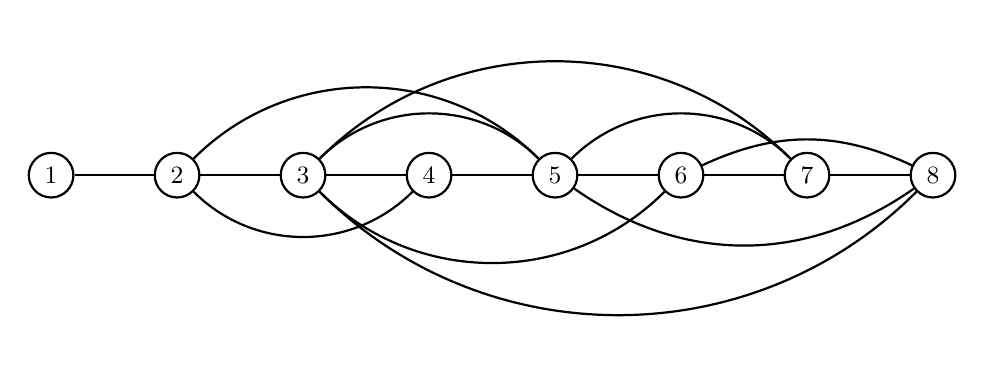
\begin{tikzpicture}[style=thick,scale=0.8]
\tikzstyle{vertex}=[draw, fill=white]
\small
\node [vertex, circle] (1) at ( 0, 0 ) {$1$};
\node [vertex, circle] (2) at (2, 0 ) {$2$};
\node [vertex, circle]  (3) at (4, 0) {$3$};
\node [vertex, circle] (4) at (6, 0) {$4$};
\node [vertex, circle] (5) at (8, 0) {$5$};
\node [vertex, circle] (6) at (10, 0) {$6$};
\node [vertex, circle] (7) at (12, 0) {$7$};
\node [vertex, circle] (8) at (14, 0) {$8$};

\draw (1) -- (2);
\draw (2) -- (3);
\draw (2) to [bend right=45] node [midway, above, sloped] {} (4);
\draw (2) to [bend left=45] node [midway, above, sloped] {} (5);
\draw (3) -- (4);
\draw (3) to [bend left=45] node [midway, above, sloped] {} (5);
\draw (3) to [bend right=45] node [midway, above, sloped] {} (6);
\draw (3) to [bend left=45] node [midway, above, sloped] {} (7);
\draw (3) to [bend right=45] node [midway, above, sloped] {} (8);
\draw (4) -- (5);
\draw (5) -- (6);
\draw (5) to [bend left=45] node [midway, above, sloped] {} (7);
\draw (5) to [bend right=35] node [midway, above, sloped] {} (8);
\draw (6) -- (7);
\draw (6) to [bend left=25] node [midway, above, sloped] {} (8);
\draw (7) -- (8);
\end{tikzpicture}

V tabeli~\tab si lahko ogledamo simulacijo.
Algoritem nam vrne optimalno pot $[1, 2, 3, 8]$, torej je $f(S) = 3$.

\begin{tabela}
\begin{tabular}{cc|cccccccccc}
$i$ & $a_i$ & $d_1$ & $d_2$ & $d_3$ & $d_4$ & $d_5$ & $d_6$ & $d_7$ & $d_8$ & $po[i]$\\ \hline
$8$ & $13$ & $\infty$ & $\infty$ & $\infty$ & $\infty$ & $\infty$ & $\infty$ & $\infty$ & $0$ & $\Null$\\
$7$ & $6$ & $\infty$ & $\infty$ & $\infty$ & $\infty$ & $\infty$ & $\infty$ & $1$ & $0$ & $8$\\
$6$ & $10$ & $\infty$ & $\infty$ & $\infty$ & $\infty$ & $\infty$ & $1$ & $1$ & $0$ & $8$\\
$5$ & $3$ & $\infty$ & $\infty$ & $\infty$ & $\infty$ & $1$ & $1$ & $1$ & $0$ & $8$\\
$4$ & $1$ & $\infty$ & $\infty$ & $\infty$ & $2$ & $1$ & $1$ & $1$ & $0$ & $5$\\
$3$ & $5$ & $\infty$ & $\infty$ & $1$ & $2$ & $1$ & $1$ & $1$ & $0$ & $8$\\
$2$ & $3$ & $\infty$ & $2$ & $1$ & $2$ & $1$ & $1$ & $1$ & $0$ & $3$\\
$1$ & $1$ & $3$ & $2$ & $1$ & $2$ & $1$ & $1$ & $1$ & $0$ & $2$\\
\end{tabular}
\podnaslov[\res{}(b)]{Potek izvajanja algoritma {\sc Skoki}}
\end{tabela}


\end{enumerate}

\end{odgovor}
\end{naloga}
